
 
 
 
 
 %%%%%%%%%%%%%%%%%%%%%%
\section{Numerical Experiments}
\label{sec:NumExp}

For our numerical experiments, we calculated normalized geodesic lengths for a variety of regression and classification tasks.  In practice, this involved training a pair of randomly initialized models to the desired test loss value/accuracy/perplexity, and then attempting to connect that pair of models via the Dynamic String Sampling algorithm.  We also tabulated the average number of ``beads'', or the number intermediate models needed by the algorithm to connect two initial models.  For all of the below experiments, the reported losses and accuracies are on a restricted test set.  For more complete architecture and implementation details, see our \href{github.com/danielfreeman11/convex-nets}{GitHub page}.


The results are broadly organized by increasing model complexity and task difficulty, from easiest to hardest.  Throughout, and remarkably, we were able to easily connect models for every dataset and architecture investigated except the one explicitly constructed counterexample discussed in Appendix \ref{symdisc}.  Qualitatively, all of the models exhibit a transition from a highly convex regime at high loss to a non-convex regime at low loss, as demonstrated by the growth of the normalized length as well as the monotonic increase in the number of required ``beads'' to form a low-loss connection.







%\begin{table}[ht]
%  \centering
%  \begin{tabular}{c@{\quad}cc}
%    & a & b \\
%    1 & 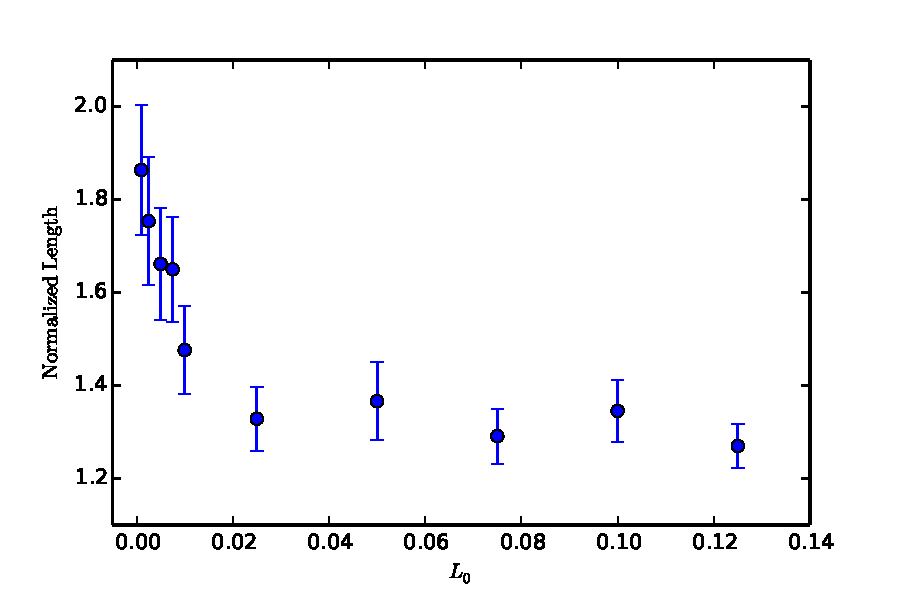
\includegraphics[width=.3\textwidth]{../Plots/normlengthquadratics}\fixedlabel{QUADRATICSfigsA}{1a} 
%      & 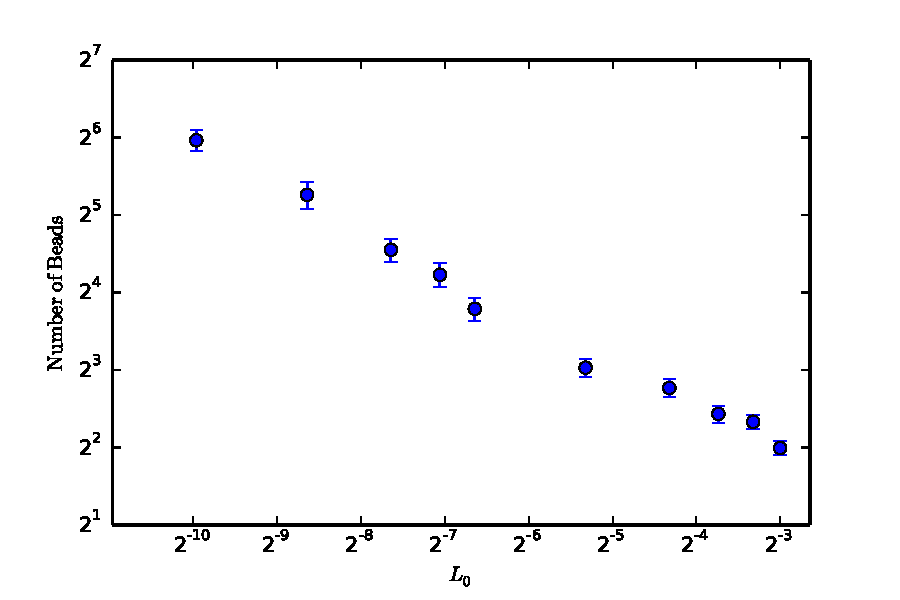
\includegraphics[width=.3\textwidth]{../Plots/numbeadsquadratics}\fixedlabel{QUADRATICSfigsB}{1b}  \\ \\
%    2 & 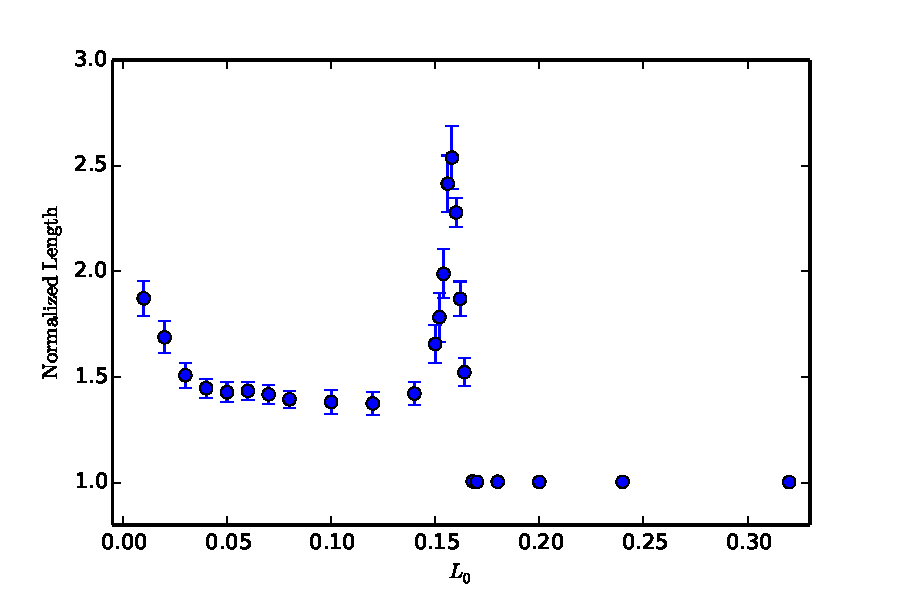
\includegraphics[width=.3\textwidth]{../Plots/normlengthcubics}\fixedlabel{CUBICSfigsA}{2a} 
%      & 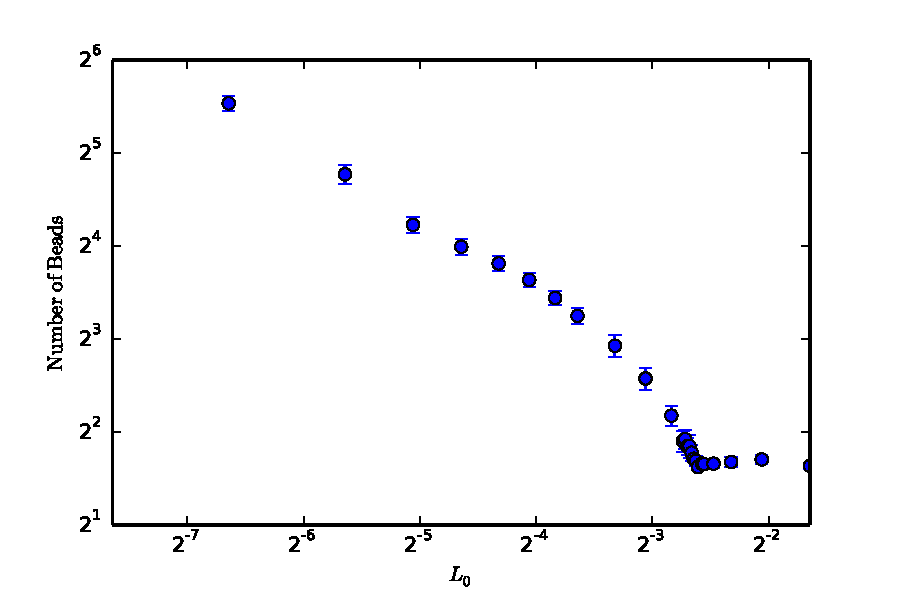
\includegraphics[width=.3\textwidth]{../Plots/numbeadscubics} \fixedlabel{CUBICSfigsB}{2b} \\ \\
%    3 & 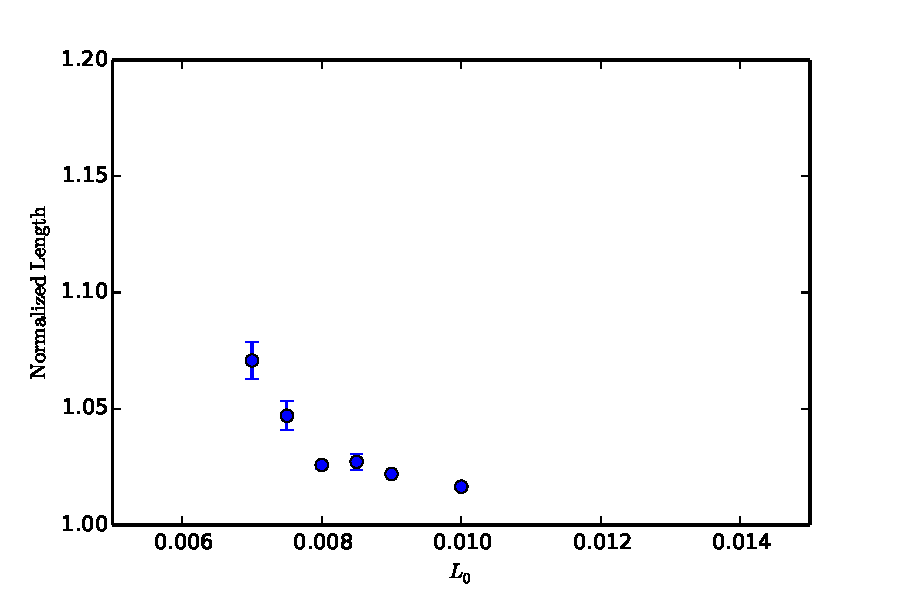
\includegraphics[width=.3\textwidth]{../Plots/normlengthMNIST}\fixedlabel{MNISTfigsA}{3a} 
%      & 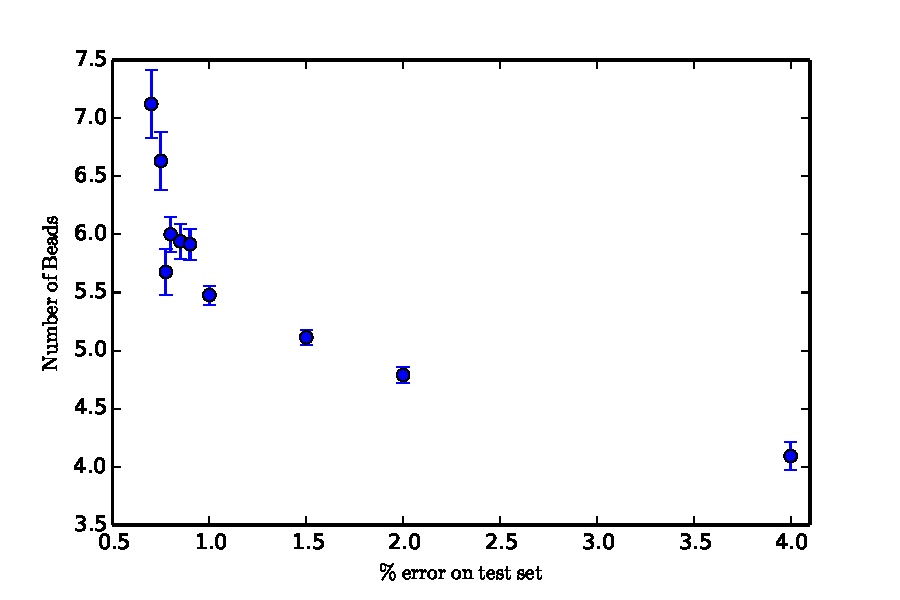
\includegraphics[width=.3\textwidth]{../Plots/numbeadsMNIST}\fixedlabel{MNISTfigsB}{3b} \\ \\
%    4 & 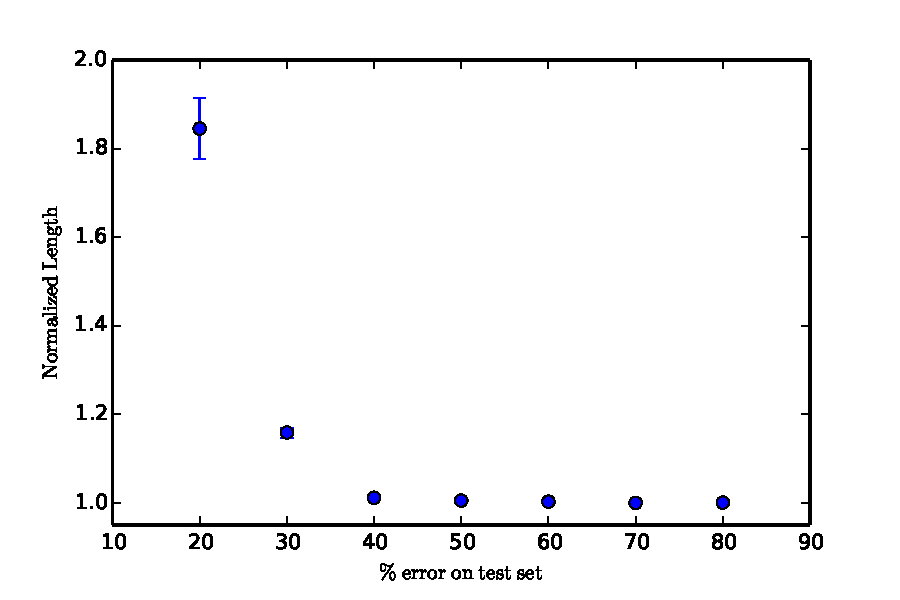
\includegraphics[width=.3\textwidth]{../Plots/normlengthCIFAR}\fixedlabel{CIFARfigsA}{4a} 
%      & 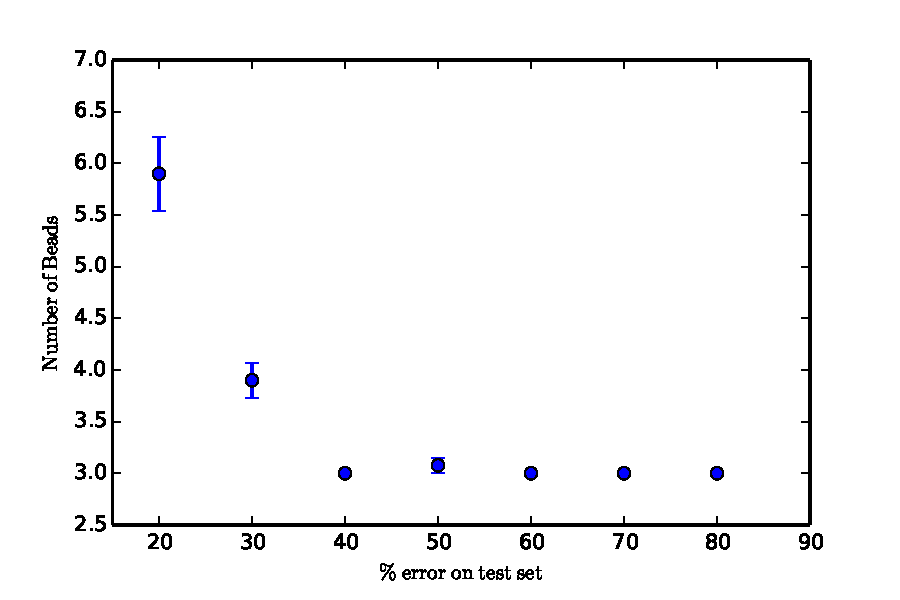
\includegraphics[width=.3\textwidth]{../Plots/numbeadsCIFAR}\fixedlabel{CIFARfigsB}{4b} \\ \\
%    5 & 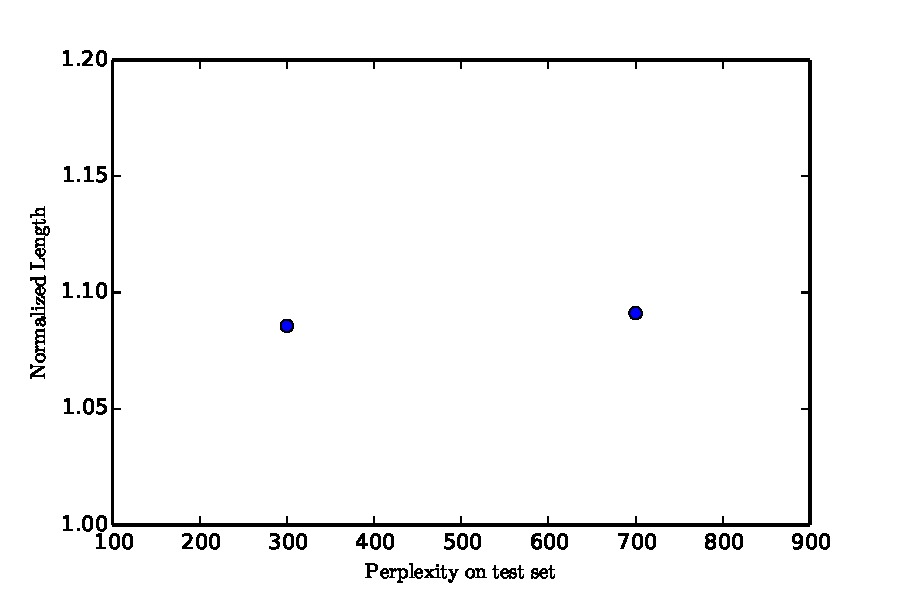
\includegraphics[width=.3\textwidth]{../Plots/normlengthPTB}\fixedlabel{PTBfigsA}{5a} 
%      & 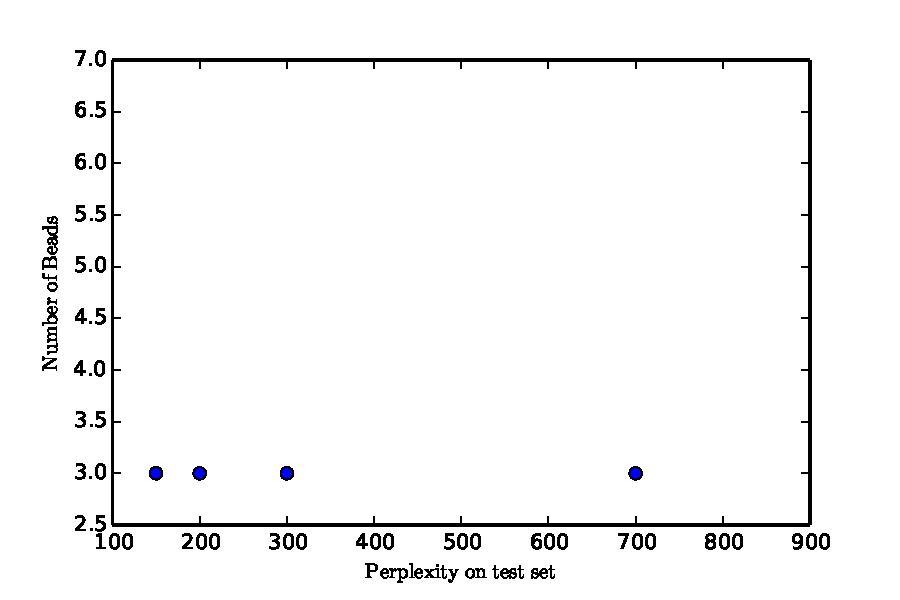
\includegraphics[width=.3\textwidth]{../Plots/numbeadsPTB}\fixedlabel{PTBfigsB}{5b}
%	 
%  \end{tabular}
%  \caption{(Column a) Average normalized geodesic length and (Column b) average number of beads versus loss. (1) \href{github.com/danielfreeman11/convex-nets/tree/master/LaunchScripts/QUADRATIC.py}{A quadratic regression task}. (2) \href{github.com/danielfreeman11/convex-nets/tree/master/LaunchScripts/CUBIC.py}{A cubic regression task}. (3) A convnet for \href{github.com/danielfreeman11/convex-nets/tree/master/LaunchScripts/MNIST.py}{MNIST}. (4) A convnet inspired by \href{www.cs.toronto.edu/\%7Ekriz/cifar.html}{Krizhevsky} for \href{github.com/danielfreeman11/convex-nets/tree/master/LaunchScripts/CIFAR10.py}{CIFAR10}. (5) \href{github.com/danielfreeman11/convex-nets/tree/master/LaunchScripts/PTBRNN.py}{A RNN} inspired by \href{arxiv.org/pdf/1409.2329.pdf}{Zaremba} for PTB next word prediction.}
%  \label{FigTable}
%\end{table}



\subsection{Polynomial Regression}
\label{sec:PolyFuncs}
%%%%%%%%%%%%%%%%%%%%%%

 We studied a 1-4-4-1 fully connected multilayer perceptron style architecture with sigmoid nonlinearities and RMSProp/ADAM optimization.  For ease-of-analysis, we restricted the training and test data to be strictly contained in the interval $x\in[0,1]$ and $f(x)\in[0,1]$.  The number of required beads, and thus the runtime of the algorithm, grew approximately as a power-law, as demonstrated in Table \ref{FigTable} Fig. 1.  We also provide a visualization of a representative connecting path between two models of equivalent power in Appendix \ref{visualization}.
 

\begin{figure} 
%\begin{figure}[h]
  \centering
%\begin{center}
%  \begin{tabular}{c@{\quad}cc}
%    & a & b \\
  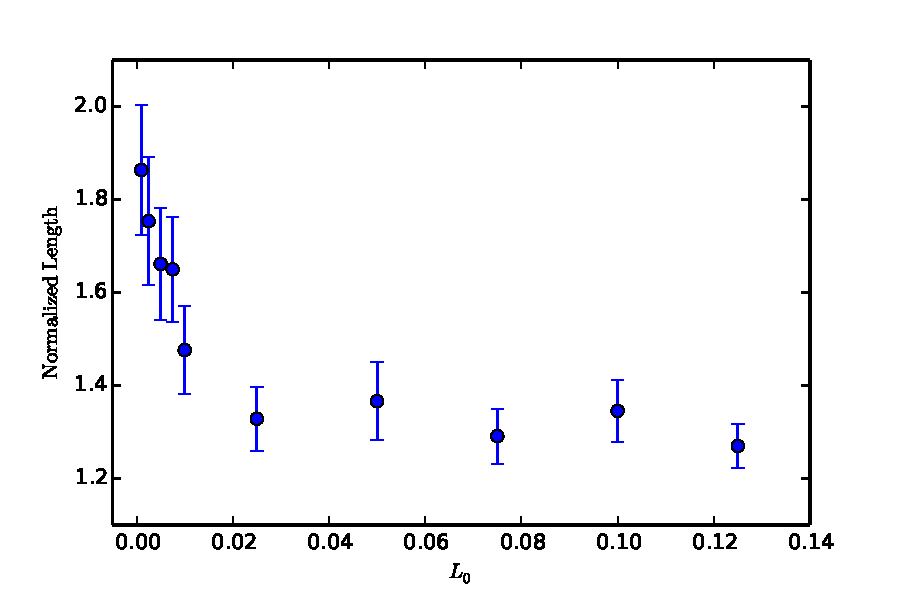
\includegraphics[width=.34\textwidth]{../Plots/normlengthquadratics}%\fixedlabel{QUADRATICSfigsA}\caption{(1a)} 
   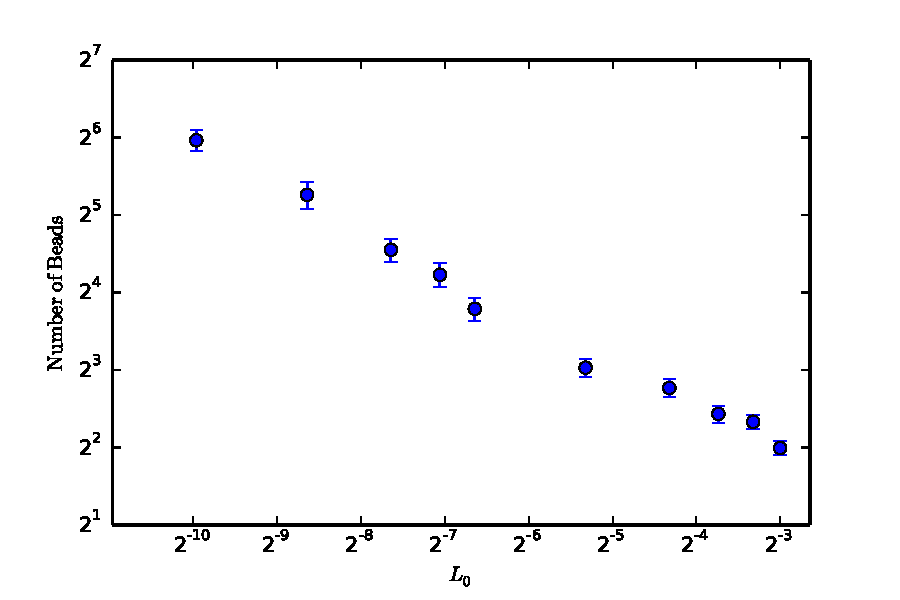
\includegraphics[width=.34\textwidth]{../Plots/numbeadsquadratics} \\ %\fixedlabel{QUADRATICSfigsB}\caption{(1b)}  \\ 
    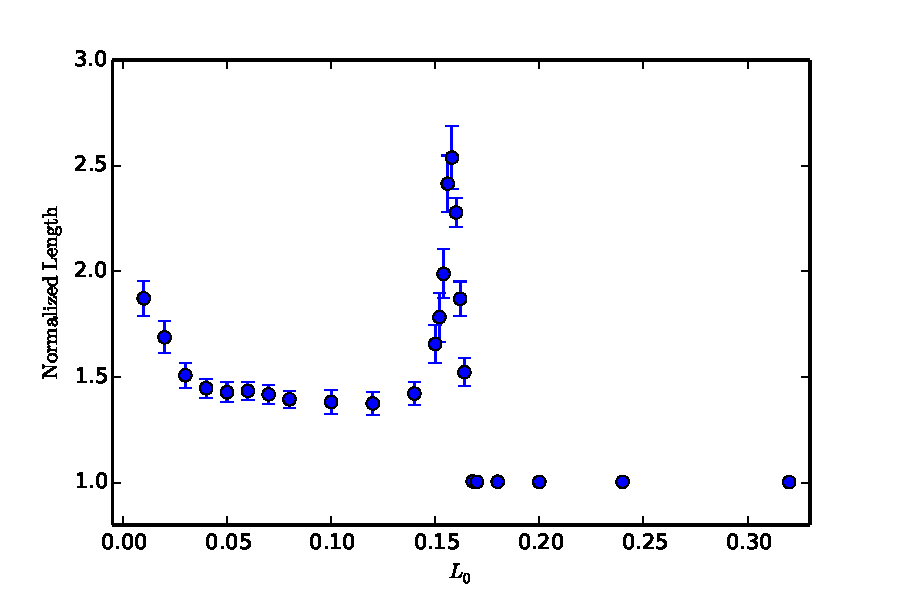
\includegraphics[width=.34\textwidth]{../Plots/normlengthcubics} %\fixedlabel{CUBICSfigsA}\caption{(2a)} 
    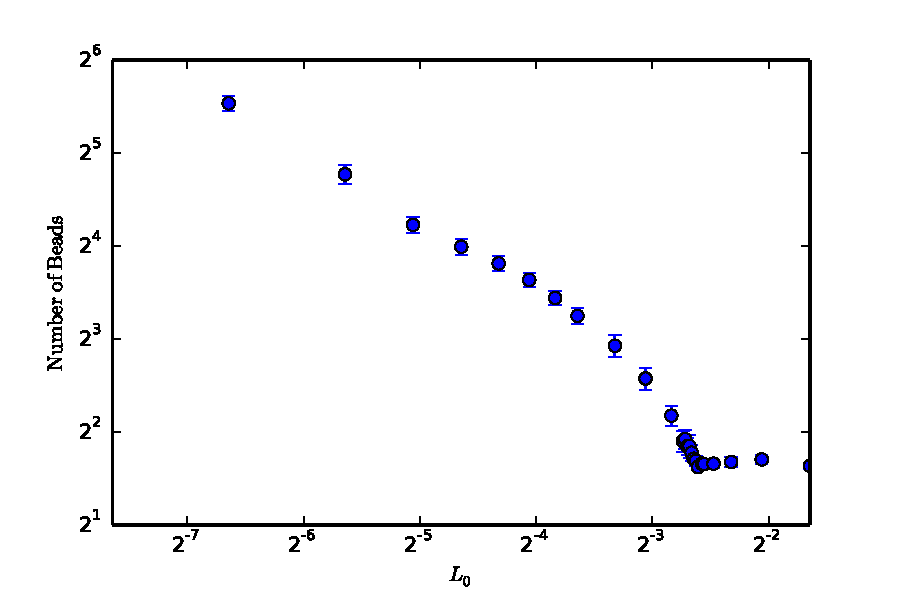
\includegraphics[width=.34\textwidth]{../Plots/numbeadscubics}\\% \fixedlabel{CUBICSfigsB}\caption{(2b)} \\
    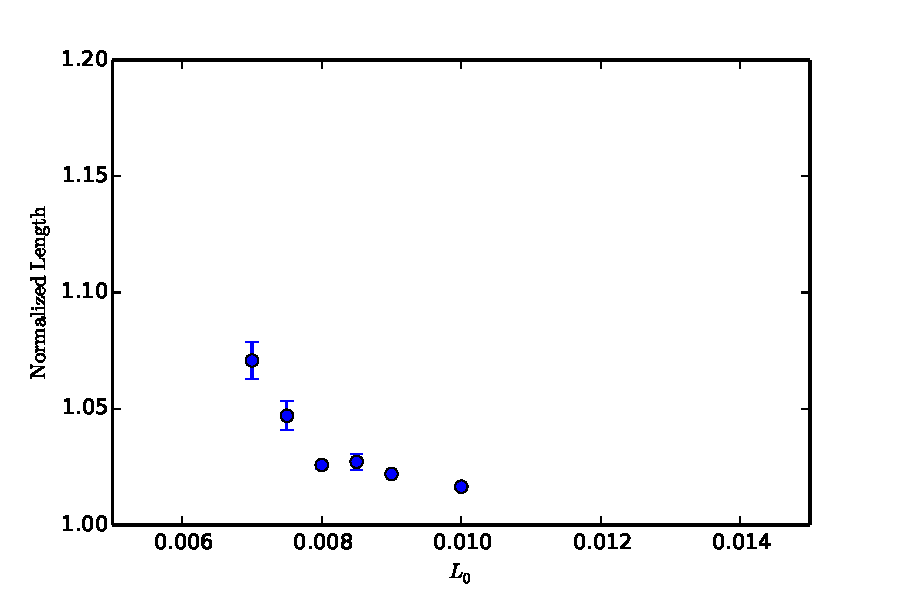
\includegraphics[width=.34\textwidth]{../Plots/normlengthMNIST}%\fixedlabel{MNISTfigsA}\caption{(3a)} 
     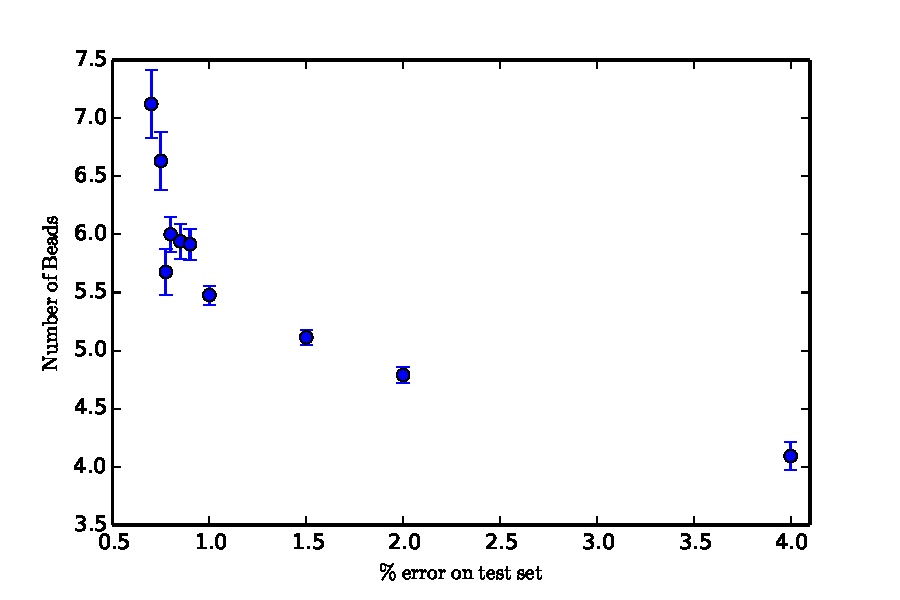
\includegraphics[width=.34\textwidth]{../Plots/numbeadsMNIST}\\% \fixedlabel{MNISTfigsB}\caption{(3b)} \\
   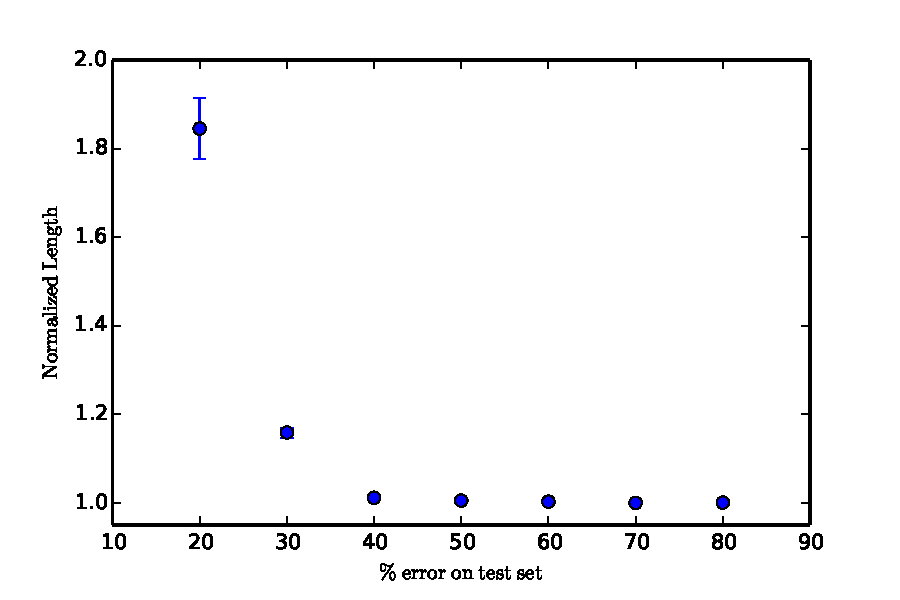
\includegraphics[width=.34\textwidth]{../Plots/normlengthCIFAR}% \fixedlabel{CIFARfigsA}\caption{(4a)} 
     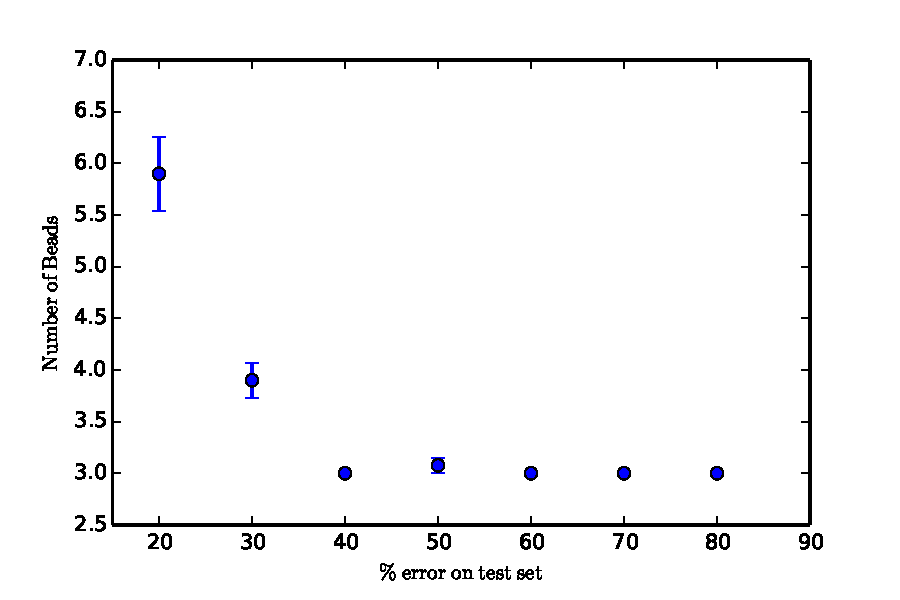
\includegraphics[width=.34\textwidth]{../Plots/numbeadsCIFAR} \\ %\fixedlabel{CIFARfigsB}\caption{(4b)} \\
   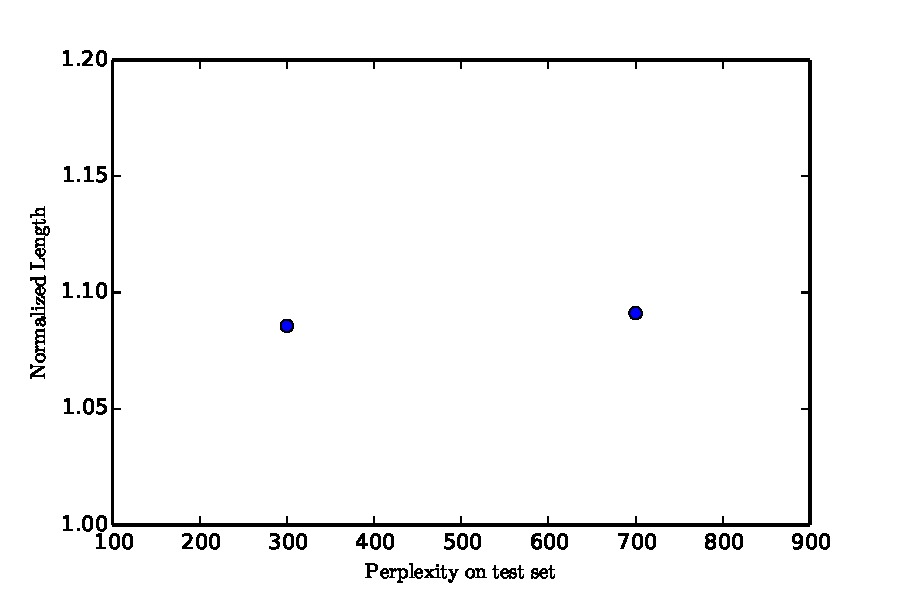
\includegraphics[width=.34\textwidth]{../Plots/normlengthPTB}% \fixedlabel{PTBfigsA}\caption{(5a)} 
   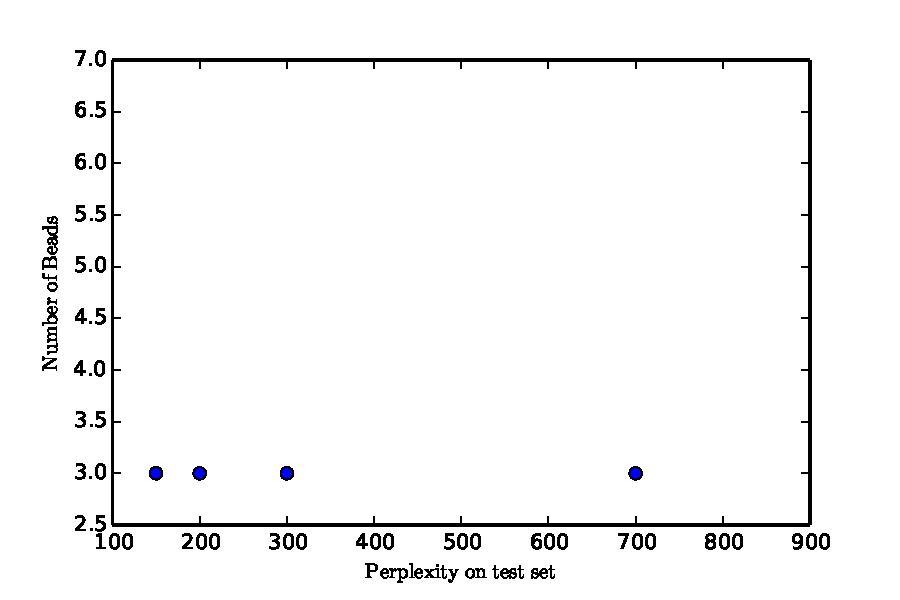
\includegraphics[width=.34\textwidth]{../Plots/numbeadsPTB} \\ %\fixedlabel{PTBfigsB}\caption{(5b)}
  \caption{(Column a) Average normalized geodesic length and (Column b) average number of beads versus loss. (1) \href{github.com/danielfreeman11/convex-nets/tree/master/LaunchScripts/QUADRATIC.py}{A quadratic regression task}. (2) \href{github.com/danielfreeman11/convex-nets/tree/master/LaunchScripts/CUBIC.py}{A cubic regression task}. (3) A convnet for \href{github.com/danielfreeman11/convex-nets/tree/master/LaunchScripts/MNIST.py}{MNIST}. (4) A convnet inspired by \href{www.cs.toronto.edu/\%7Ekriz/cifar.html}{Krizhevsky} for \href{github.com/danielfreeman11/convex-nets/tree/master/LaunchScripts/CIFAR10.py}{CIFAR10}. (5) \href{github.com/danielfreeman11/convex-nets/tree/master/LaunchScripts/PTBRNN.py}{A RNN} inspired by \href{arxiv.org/pdf/1409.2329.pdf}{Zaremba} for PTB next word prediction.}
  \label{FigTable}
\end{figure}
%\end{center}

 
 The cubic regression task exhibits an interesting feature around $L_0=.15$ in Table \ref{FigTable} Fig. 2, where the normalized length spikes, but the number of required beads remains low.  Up until this point, the cubic model is strongly convex, so this first spike seems to indicate the onset of non-convex behavior and a concomitant radical change in the geometry of the loss surface for lower loss.
  
 
%%%%%%%%%%%%%%%%%%%%%%
\subsection{Convolutional Neural Networks}
\label{sec:CNN}
%%%%%%%%%%%%%%%%%%%%%%

 To test the algorithm on larger architectures, we ran it on the MNIST hand written digit recognition task as well as the CIFAR10 image recognition task, indicated in Table \ref{FigTable}, Figs. 3 and 4.  Again, the data exhibits strong qualitative similarity with the previous models: normalized length remains low until a threshold loss value, after which it grows approximately as a power law.  Interestingly, the MNIST dataset exhibits very low normalized length, even for models nearly at the state of the art in classification power, in agreement with the folk-understanding that MNIST is highly convex and/or ``easy''.  The CIFAR10 dataset, however, exhibits large non-convexity, even at the modest test accuracy of 80\%.


%%%%%%%%%%%%%%%%%%%%%%
\subsection{Recurrent Neural Networks}
%%%%%%%%%%%%%%%%%%%%%%

 To gauge the generalizability of our algorithm, we also applied it to an LSTM architecture for solving the next word prediction task on the PTB dataset, depicted in Table \ref{FigTable} Fig. 5.  Noteably, even for a radically different architecture, loss function, and data set, the normalized lengths produced by the DSS algorithm recapitulate the same qualitative features seen in the above datasets---i.e., models can be easily connected at high perplexity, and the normalized length grows at lower and lower perplexity after a threshold value, indicating an onset of increased non-convexity of the loss surface.



